\section{Motivation and Scope}

There has been a strong desire for a more space- and/or runtime-efficient
representation for \code{map} among C++ users for some time now.  This has
motivated discussions among the members of SG14, numerous articles and talks,
and an implementation in Boost, \code{boost::container::flat_map}.  Virtually
everyone who makes games, embedded, or system software in C++ uses the Boost
implementation or one that they rolled themselves.\\

Here are some numbers that show why.  The graphs that follow show runtimes for
different \code{map}-like associative containers.  The containers used are
Boost.FlatMap, \code{std::map}, and two thin wrappers over a sorted
\code{std::vector}; the ``custom pair'' version of the sorted
\code{std::vector} uses a simple struct instead of \code{std::pair} for its
value type.  All containers use an \code{int} as the key type and an
\code{int} or a struct with 5 \code{double}s for the value type.

These first three graphs cover the int-value-type case.  The first
graph shows insertion of N elements with random keys; the second shows full
iteration across all N elements; and the third shows erasure of all N
elements, by the keys used in the original insertions.

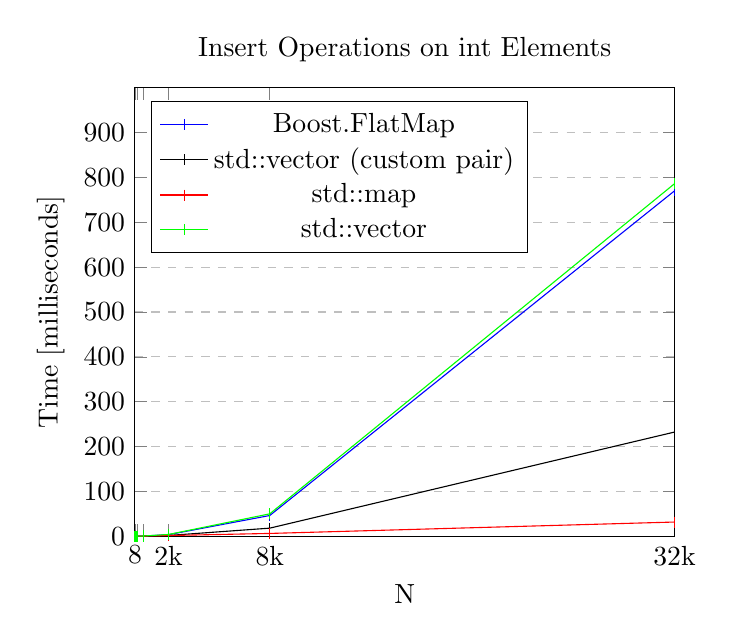
\begin{tikzpicture}
    \begin{axis}[
        title={Insert Operations on int Elements},
        xlabel={N},
        ylabel={Time [milliseconds]},
        xmin=0, xmax=32768.0,
        ymin=0, ymax=1000.0,
        xtick={8,32,128,512,2048,8192,32768},
        xticklabels={8,,,,2k,8k,32k},
        ytick={0.0,100.0,200.0,300.0,400.0,500.0,600.0,700.0,800.0,900.0},
        legend pos=north west,
        ymajorgrids=true,
        grid style=dashed,
        scaled x ticks=false,
        legend entries={Boost.FlatMap,std::vector (custom pair),std::map,std::vector},
        ]

    \addplot[color=blue,mark=|,]
        coordinates {(8,0.0061)(32,0.009)(128,0.0466)(512,0.3269)(2048,3.4296)(8192,46.1462)(32768,770.289)};

    \addplot[color=black,mark=|,]
        coordinates {(8,0.0051)(32,0.0133)(128,0.1292)(512,0.2641)(2048,1.6346)(8192,17.9527)(32768,232.288)};

    \addplot[color=red,mark=|,]
        coordinates {(8,0.0084)(32,0.0187)(128,0.0794)(512,0.3573)(2048,1.4816)(8192,6.1507)(32768,31.5773)};

    \addplot[color=green,mark=|,]
        coordinates {(8,0.0045)(32,0.0135)(128,0.0535)(512,0.3669)(2048,3.8914)(8192,49.8729)(32768,786.225)};

    \end{axis}
\end{tikzpicture}

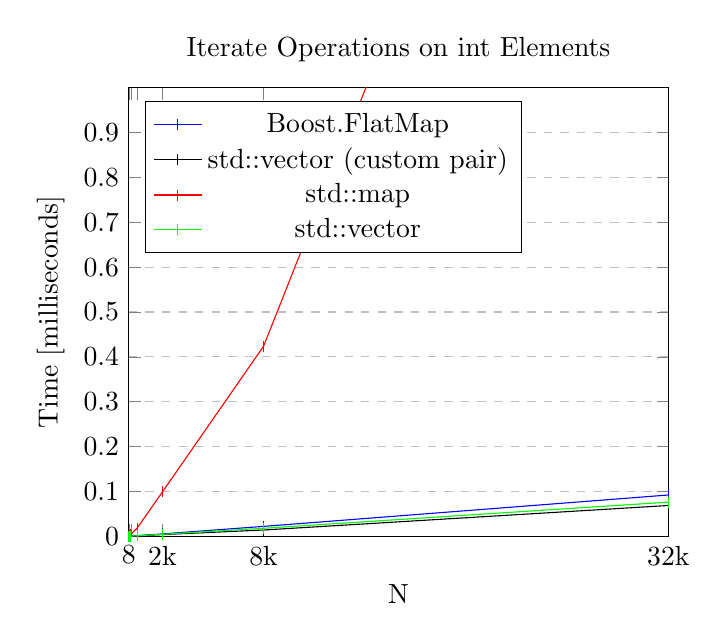
\begin{tikzpicture}
    \begin{axis}[
        title={Iterate Operations on int Elements},
        xlabel={N},
        ylabel={Time [milliseconds]},
        xmin=0, xmax=32768.0,
        ymin=0, ymax=1.0,
        xtick={8,32,128,512,2048,8192,32768},
        xticklabels={8,,,,2k,8k,32k},
        ytick={0.0,0.1,0.2,0.3,0.4,0.5,0.6,0.7,0.8,0.9},
        legend pos=north west,
        ymajorgrids=true,
        grid style=dashed,
        scaled x ticks=false,
        legend entries={Boost.FlatMap,std::vector (custom pair),std::map,std::vector},
        ]

    \addplot[color=blue,mark=|,]
        coordinates {(8,0)(32,0)(128,0.0006)(512,0.0012)(2048,0.0051)(8192,0.0219)(32768,0.0919)};

    \addplot[color=black,mark=|,]
        coordinates {(8,0)(32,0.0003)(128,0.0003)(512,0.0009)(2048,0.0036)(8192,0.0138)(32768,0.0685)};

    \addplot[color=red,mark=|,]
        coordinates {(8,0.0003)(32,0.0012)(128,0.0042)(512,0.018)(2048,0.0988)(8192,0.4239)(32768,2.7052)};

    \addplot[color=green,mark=|,]
        coordinates {(8,0.0003)(32,0)(128,0.0003)(512,0.0009)(2048,0.0042)(8192,0.0177)(32768,0.076)};

    \end{axis}
\end{tikzpicture}

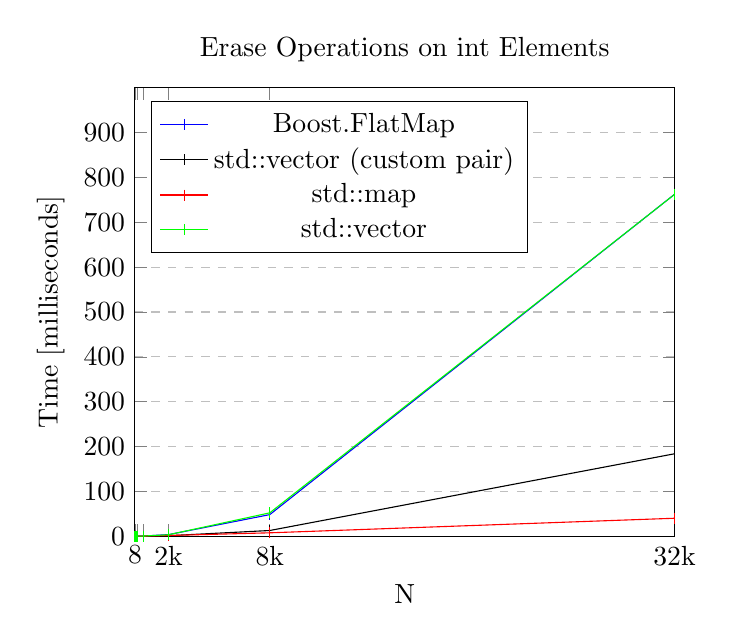
\begin{tikzpicture}
    \begin{axis}[
        title={Erase Operations on int Elements},
        xlabel={N},
        ylabel={Time [milliseconds]},
        xmin=0, xmax=32768.0,
        ymin=0, ymax=1000.0,
        xtick={8,32,128,512,2048,8192,32768},
        xticklabels={8,,,,2k,8k,32k},
        ytick={0.0,100.0,200.0,300.0,400.0,500.0,600.0,700.0,800.0,900.0},
        legend pos=north west,
        ymajorgrids=true,
        grid style=dashed,
        scaled x ticks=false,
        legend entries={Boost.FlatMap,std::vector (custom pair),std::map,std::vector},
        ]

    \addplot[color=blue,mark=|,]
        coordinates {(8,0.0012)(32,0.0057)(128,0.0438)(512,0.3305)(2048,3.5648)(8192,48.1307)(32768,762.534)};

    \addplot[color=black,mark=|,]
        coordinates {(8,0.0015)(32,0.0048)(128,0.0526)(512,0.1767)(2048,1.0979)(8192,12.7021)(32768,183.828)};

    \addplot[color=red,mark=|,]
        coordinates {(8,0.003)(32,0.0129)(128,0.0622)(512,0.3152)(2048,1.5481)(8192,7.5319)(32768,40.0228)};

    \addplot[color=green,mark=|,]
        coordinates {(8,0.0006)(32,0.0042)(128,0.0336)(512,0.2899)(2048,3.2577)(8192,52.0944)(32768,762.365)};

    \end{axis}
\end{tikzpicture}


These next three graphs are just like the preceding ones, but cover the
struct-value-type case.

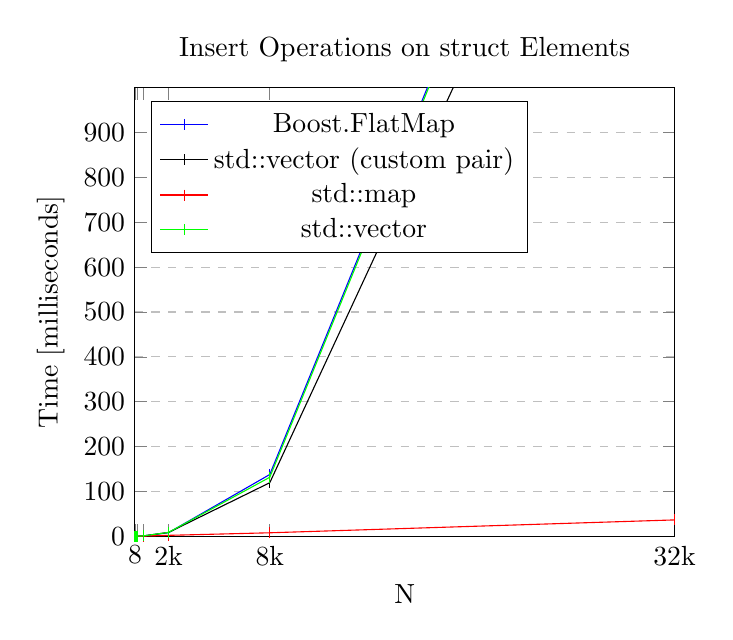
\begin{tikzpicture}
    \begin{axis}[
        title={Insert Operations on struct Elements},
        xlabel={N},
        ylabel={Time [milliseconds]},
        xmin=0, xmax=32768.0,
        ymin=0, ymax=1000.0,
        xtick={8,32,128,512,2048,8192,32768},
        xticklabels={8,,,,2k,8k,32k},
        ytick={0.0,100.0,200.0,300.0,400.0,500.0,600.0,700.0,800.0,900.0},
        legend pos=north west,
        ymajorgrids=true,
        grid style=dashed,
        scaled x ticks=false,
        legend entries={Boost.FlatMap,std::vector (custom pair),std::map,std::vector},
        ]

    \addplot[color=blue,mark=|,]
        coordinates {(8,0.006)(32,0.0138)(128,0.0712)(512,0.5911)(2048,7.9643)(8192,137.592)(32768,2353.55)};

    \addplot[color=black,mark=|,]
        coordinates {(8,0.0069)(32,0.0319)(128,0.1241)(512,0.5962)(2048,8.3777)(8192,119.313)(32768,2063.73)};

    \addplot[color=red,mark=|,]
        coordinates {(8,0.0105)(32,0.0186)(128,0.1028)(512,0.3558)(2048,1.8993)(8192,7.6045)(32768,36.3057)};

    \addplot[color=green,mark=|,]
        coordinates {(8,0.0075)(32,0.0198)(128,0.082)(512,0.6776)(2048,8.5222)(8192,131.445)(32768,2344.63)};

    \end{axis}
\end{tikzpicture}

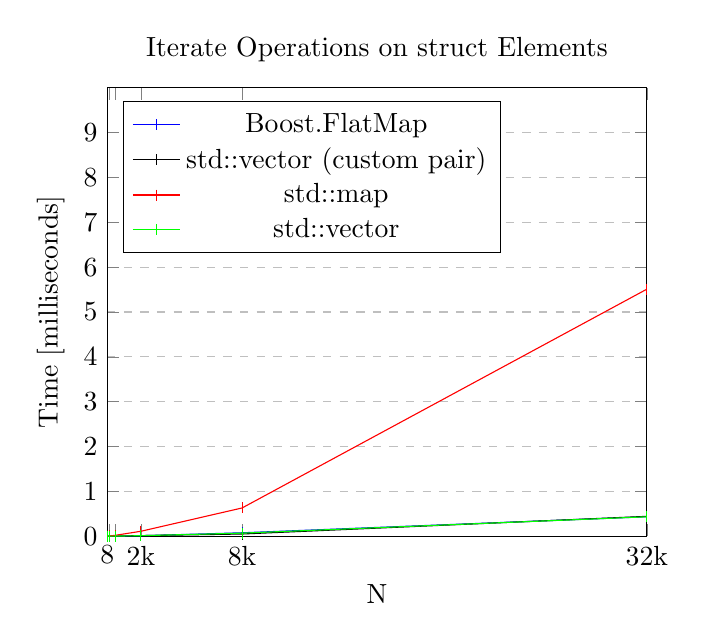
\begin{tikzpicture}
    \begin{axis}[
        title={Iterate Operations on struct Elements},
        xlabel={N},
        ylabel={Time [milliseconds]},
        xmin=0, xmax=32768.0,
        ymin=0, ymax=10.0,
        xtick={8,32,128,512,2048,8192,32768},
        xticklabels={8,,,,2k,8k,32k},
        ytick={0.0,1.0,2.0,3.0,4.0,5.0,6.0,7.0,8.0,9.0},
        legend pos=north west,
        ymajorgrids=true,
        grid style=dashed,
        scaled x ticks=false,
        legend entries={Boost.FlatMap,std::vector (custom pair),std::map,std::vector},
        ]

    \addplot[color=blue,mark=|,]
        coordinates {(8,0.0003)(32,0)(128,0.0003)(512,0.0015)(2048,0.0108)(8192,0.0761)(32768,0.4339)};

    \addplot[color=black,mark=|,]
        coordinates {(8,0)(32,0)(128,0.0006)(512,0.0021)(2048,0.0129)(8192,0.0487)(32768,0.4429)};

    \addplot[color=red,mark=|,]
        coordinates {(8,0.0003)(32,0.0012)(128,0.0045)(512,0.0207)(2048,0.11)(8192,0.6298)(32768,5.5097)};

    \addplot[color=green,mark=|,]
        coordinates {(8,0)(32,0)(128,0.0003)(512,0.0021)(2048,0.0114)(8192,0.0682)(32768,0.4327)};

    \end{axis}
\end{tikzpicture}

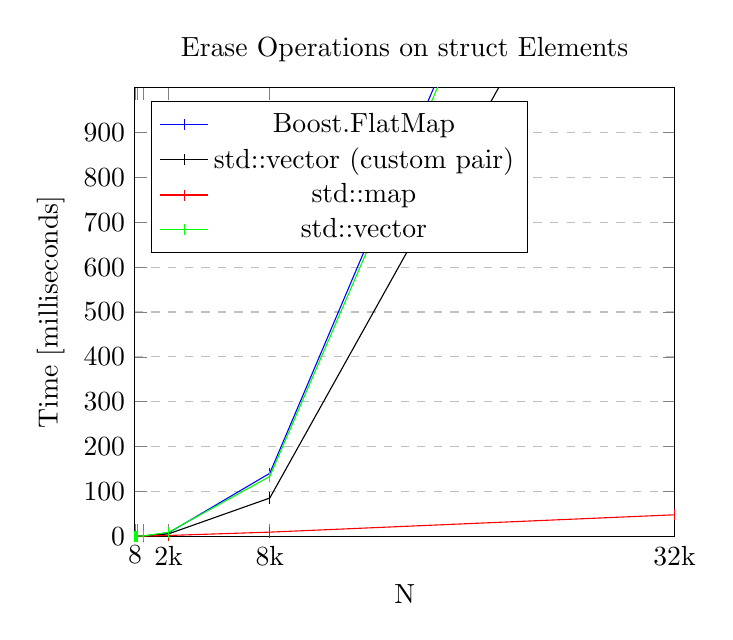
\begin{tikzpicture}
    \begin{axis}[
        title={Erase Operations on struct Elements},
        xlabel={N},
        ylabel={Time [milliseconds]},
        xmin=0, xmax=32768.0,
        ymin=0, ymax=1000.0,
        xtick={8,32,128,512,2048,8192,32768},
        xticklabels={8,,,,2k,8k,32k},
        ytick={0.0,100.0,200.0,300.0,400.0,500.0,600.0,700.0,800.0,900.0},
        legend pos=north west,
        ymajorgrids=true,
        grid style=dashed,
        scaled x ticks=false,
        legend entries={Boost.FlatMap,std::vector (custom pair),std::map,std::vector},
        ]

    \addplot[color=blue,mark=|,]
        coordinates {(8,0.0015)(32,0.0072)(128,0.0529)(512,0.5513)(2048,7.4591)(8192,140.312)(32768,2262.71)};

    \addplot[color=black,mark=|,]
        coordinates {(8,0.0012)(32,0.0054)(128,0.0346)(512,0.3449)(2048,5.2023)(8192,85.1265)(32768,1703.69)};

    \addplot[color=red,mark=|,]
        coordinates {(8,0.003)(32,0.0118)(128,0.0604)(512,0.3155)(2048,1.6225)(8192,9.0607)(32768,47.7431)};

    \addplot[color=green,mark=|,]
        coordinates {(8,0.0009)(32,0.0051)(128,0.0439)(512,0.5153)(2048,8.7305)(8192,133.166)(32768,2226.12)};

    \end{axis}
\end{tikzpicture}

